\chaptr{Anexos}{anexos}

% ----------------------------------------------------------------------------------------------- %

\sect{Anexo A: Pila del producto}{anexoA}

Durante el desarrollo del proyecto se han realizado una serie de tareas, para las cuales se ha utilizado la
herramienta \boldFont{Notion}.
Esta herramienta proporciona una interfaz muy sencilla para la creación de tareas, con la
posibilidad de añadir etiquetas, asignar responsables, añadir comentarios a cada una de ellas,
entre otras funcionalidades.
A continuación, se incluye el fichero pdf generado por Notion con la pila del producto completa.\ Además, se puede
consultar la pila del producto de una manera más interactiva en el siguiente enlace:
\href{https://scastd00.notion.site/9c59c2812d8b440faa453924fef2f320?v=20f7c2f47dd64574ac57713e8efe2718}
{https://scastd00.notion.site/9c59c2812d8b440faa453924fef2f3
20?v=20f7c2f47dd64574ac57713e8efe2718}

% Generar el pdf a 57% de tamaño para que quepa el ancho de página incluyendo las notas de Notion.
\label{anx:product-backlog-notion}
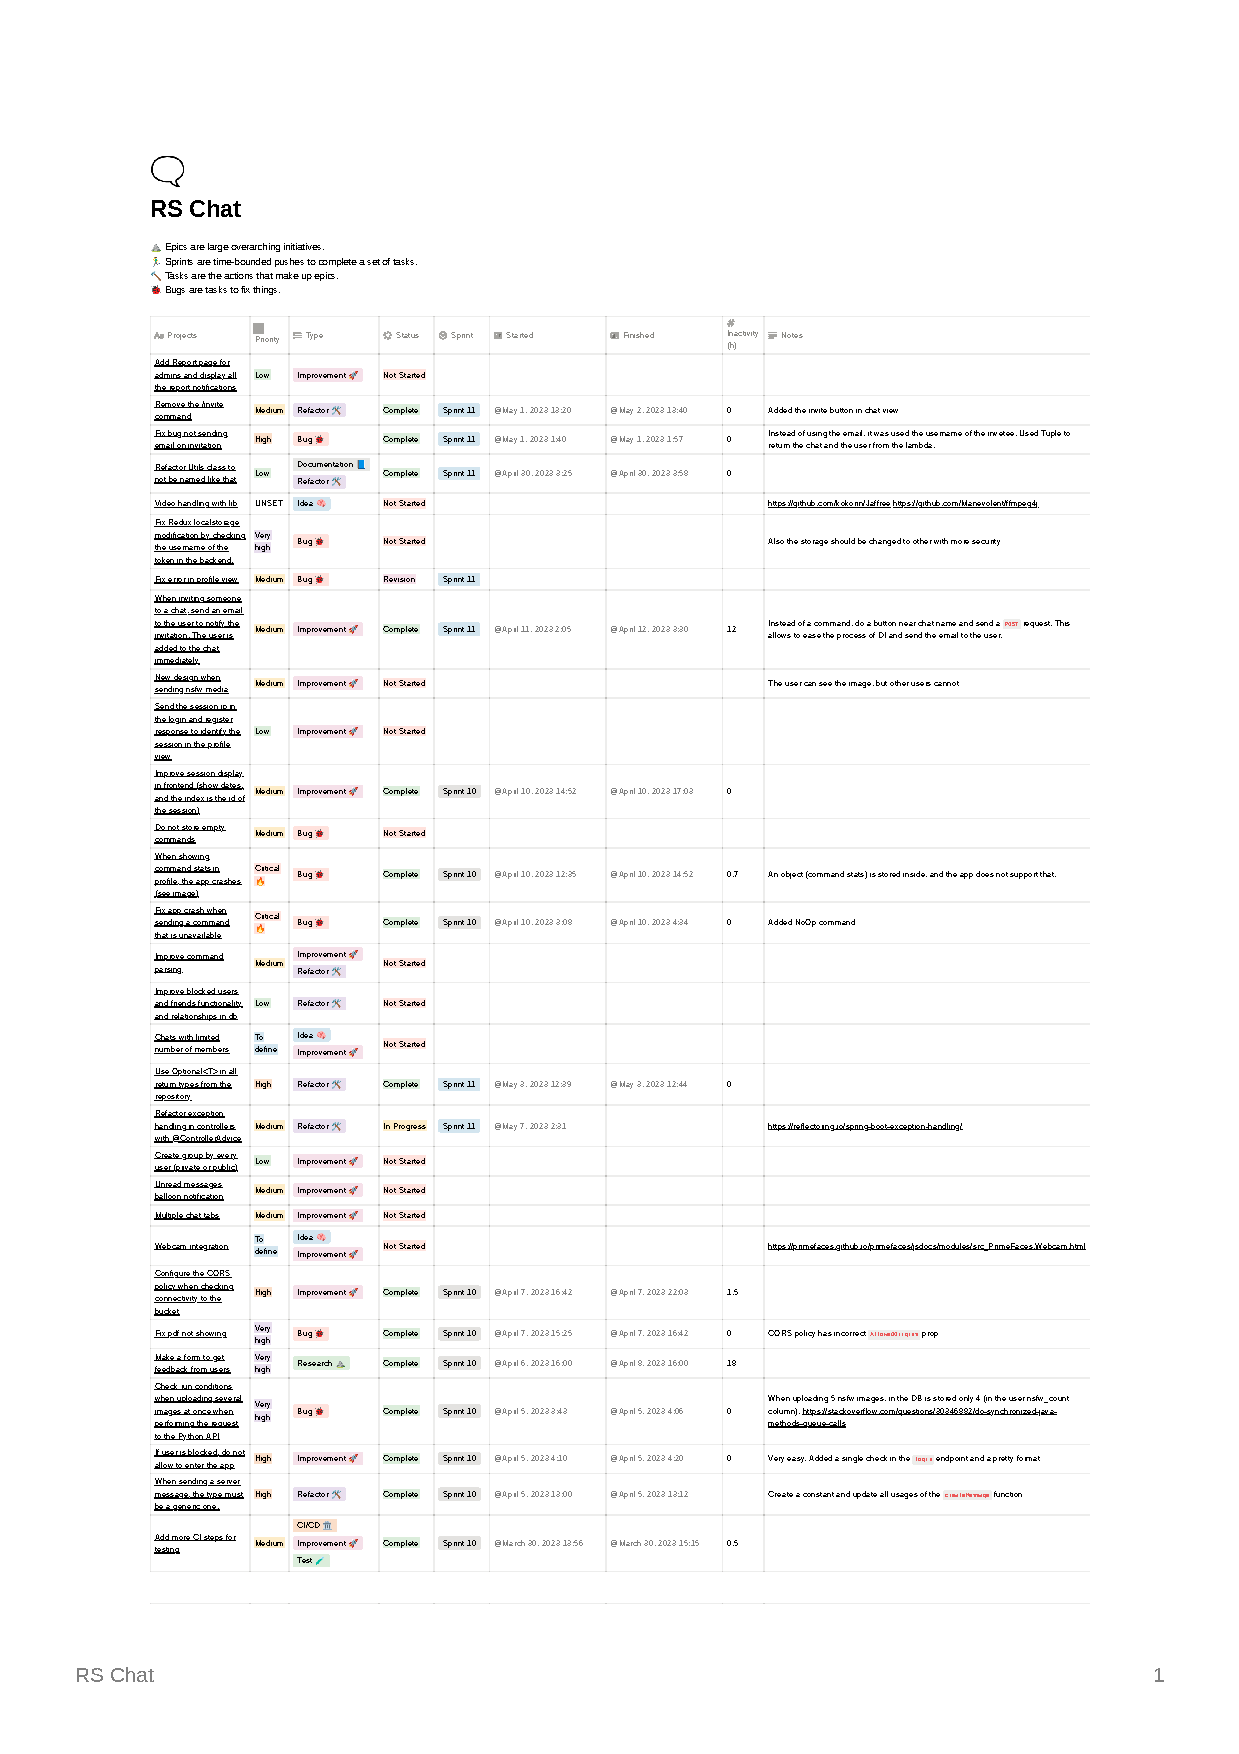
\includepdf[pages=-]{anexos/TareasNotion.pdf}

% ----------------------------------------------------------------------------------------------- %

\sect{Anexo B: Encuesta de satisfacción}{anexoB}

La encuesta de satisfacción realizada a los usuarios se puede visitar en el siguiente enlace:
\href{https://tally.so/r/31XyPQ}{https://tally.so/r/31XyPQ}
\label{anx:encuesta-satisfaccion}

% ----------------------------------------------------------------------------------------------- %

\sect{Anexo C: Diagramas de Gantt}{anexoC}

En esta sección se incluye el diagrama de Gantt completo del proyecto y el enlace a la hoja de cálculo de Google
Sheets con la que se ha generado.\ Además, esta contiene la pila del producto con las tareas completas y los diagramas
de Gantt de cada sprint de manera individual en hojas separadas.\ El enlace a la hoja de cálculo es el siguiente:
\href{https://docs.google.com/spreadsheets/d/1GOffJpsR0vORsQYvTrbWj72jmHIJvB0UMZqahqMcR-s/edit?usp=sharing}
{https://docs.google.com/spreadsheets/d/1GOffJpsR0vORsQYvTrbWj72jmHIJvB0U\\MZqahqMcR-s/edit?usp=sharing}

\label{anx:gantt}
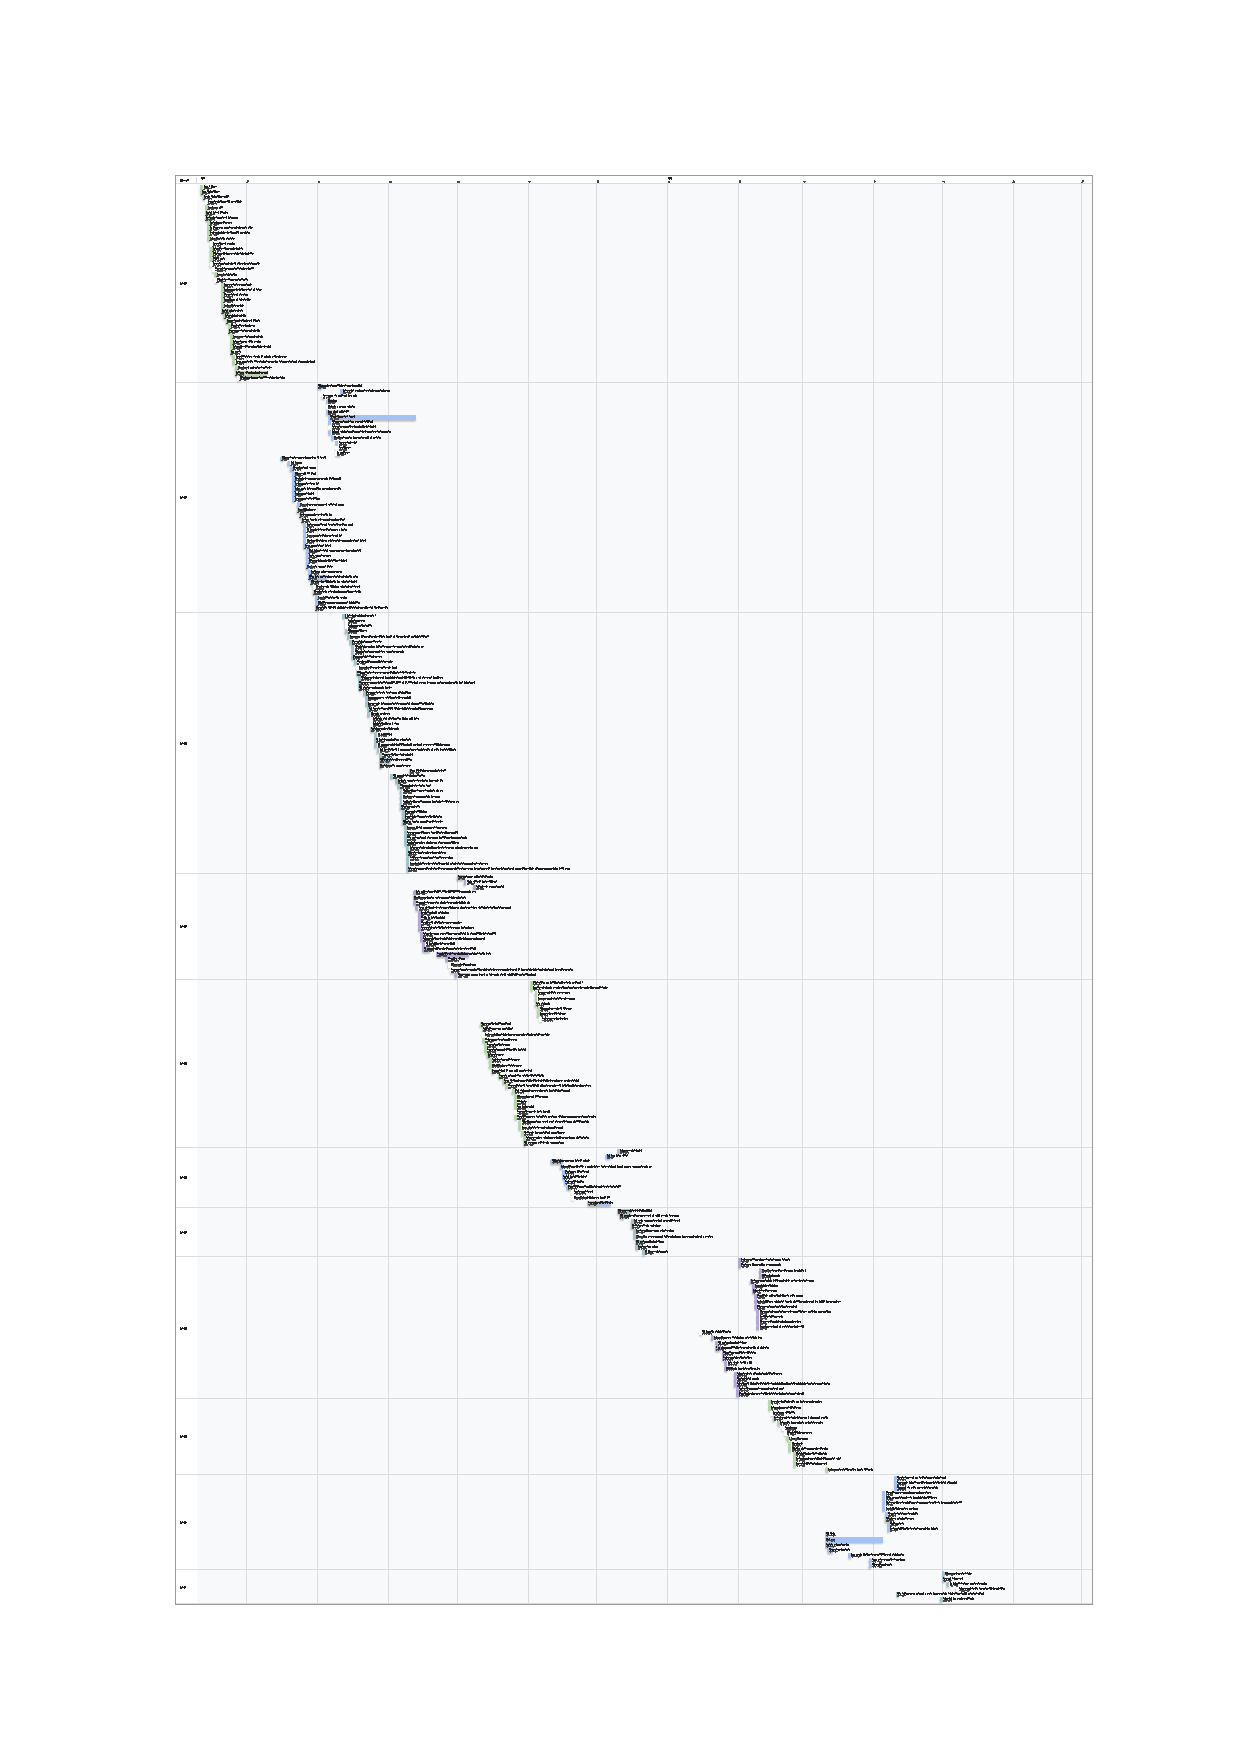
\includepdf[pages=-]{anexos/TodosLosSprints.pdf}

% ----------------------------------------------------------------------------------------------- %

\sect{Anexo D: Manual de usuario}{anexoD}

En esta sección se incluye el manual de usuario completo de la aplicación.\ Se incluye la funcionalidad para todos
los roles de usuario, tanto para el administrador como para el usuario normal.\ Además, se incluye la funcionalidad
de la aplicación web.\ El manual de usuario se ha generado en formato pdf a partir de Google Docs.

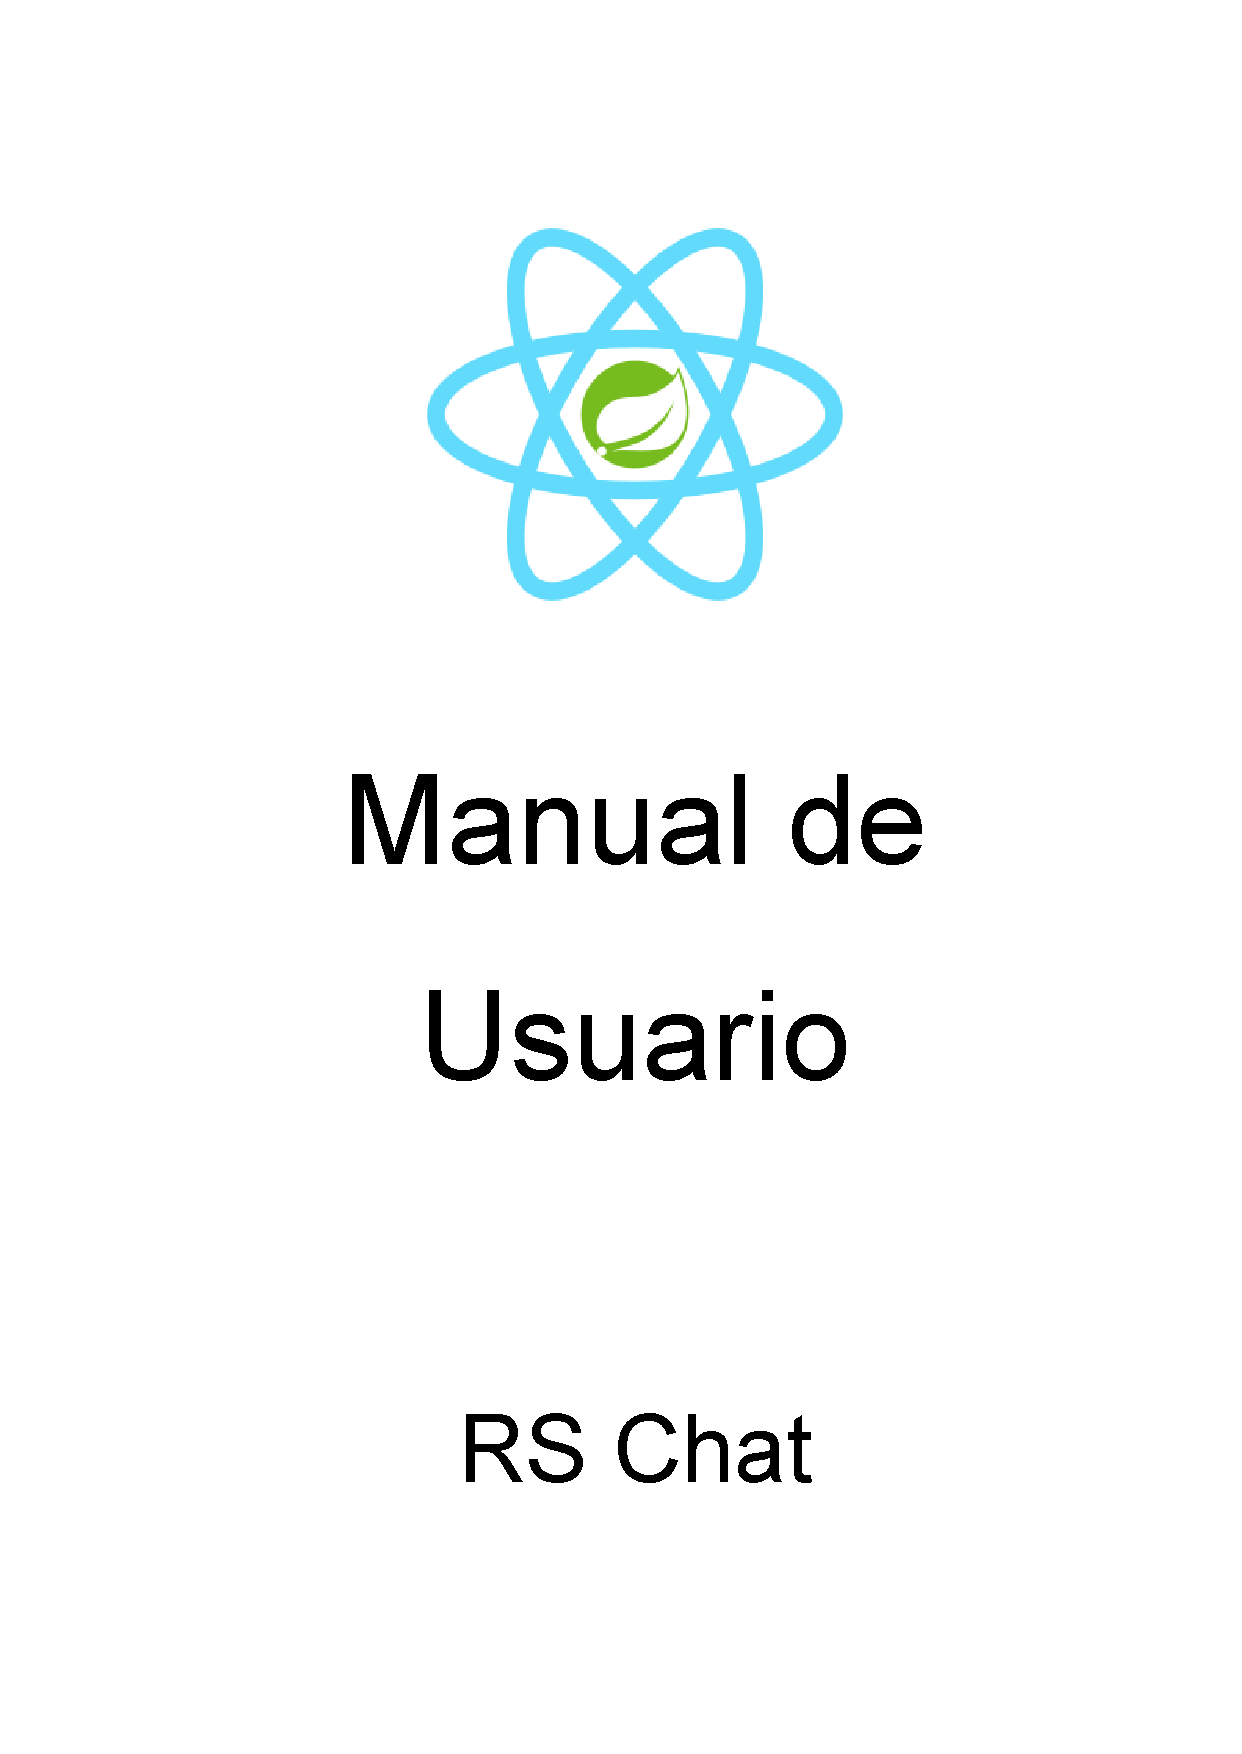
\includepdf[pages=-]{anexos/ManualUsuarioRSChat.pdf}
